\begin{tikzpicture}[remember picture,overlay]
    \node at (current page.center) {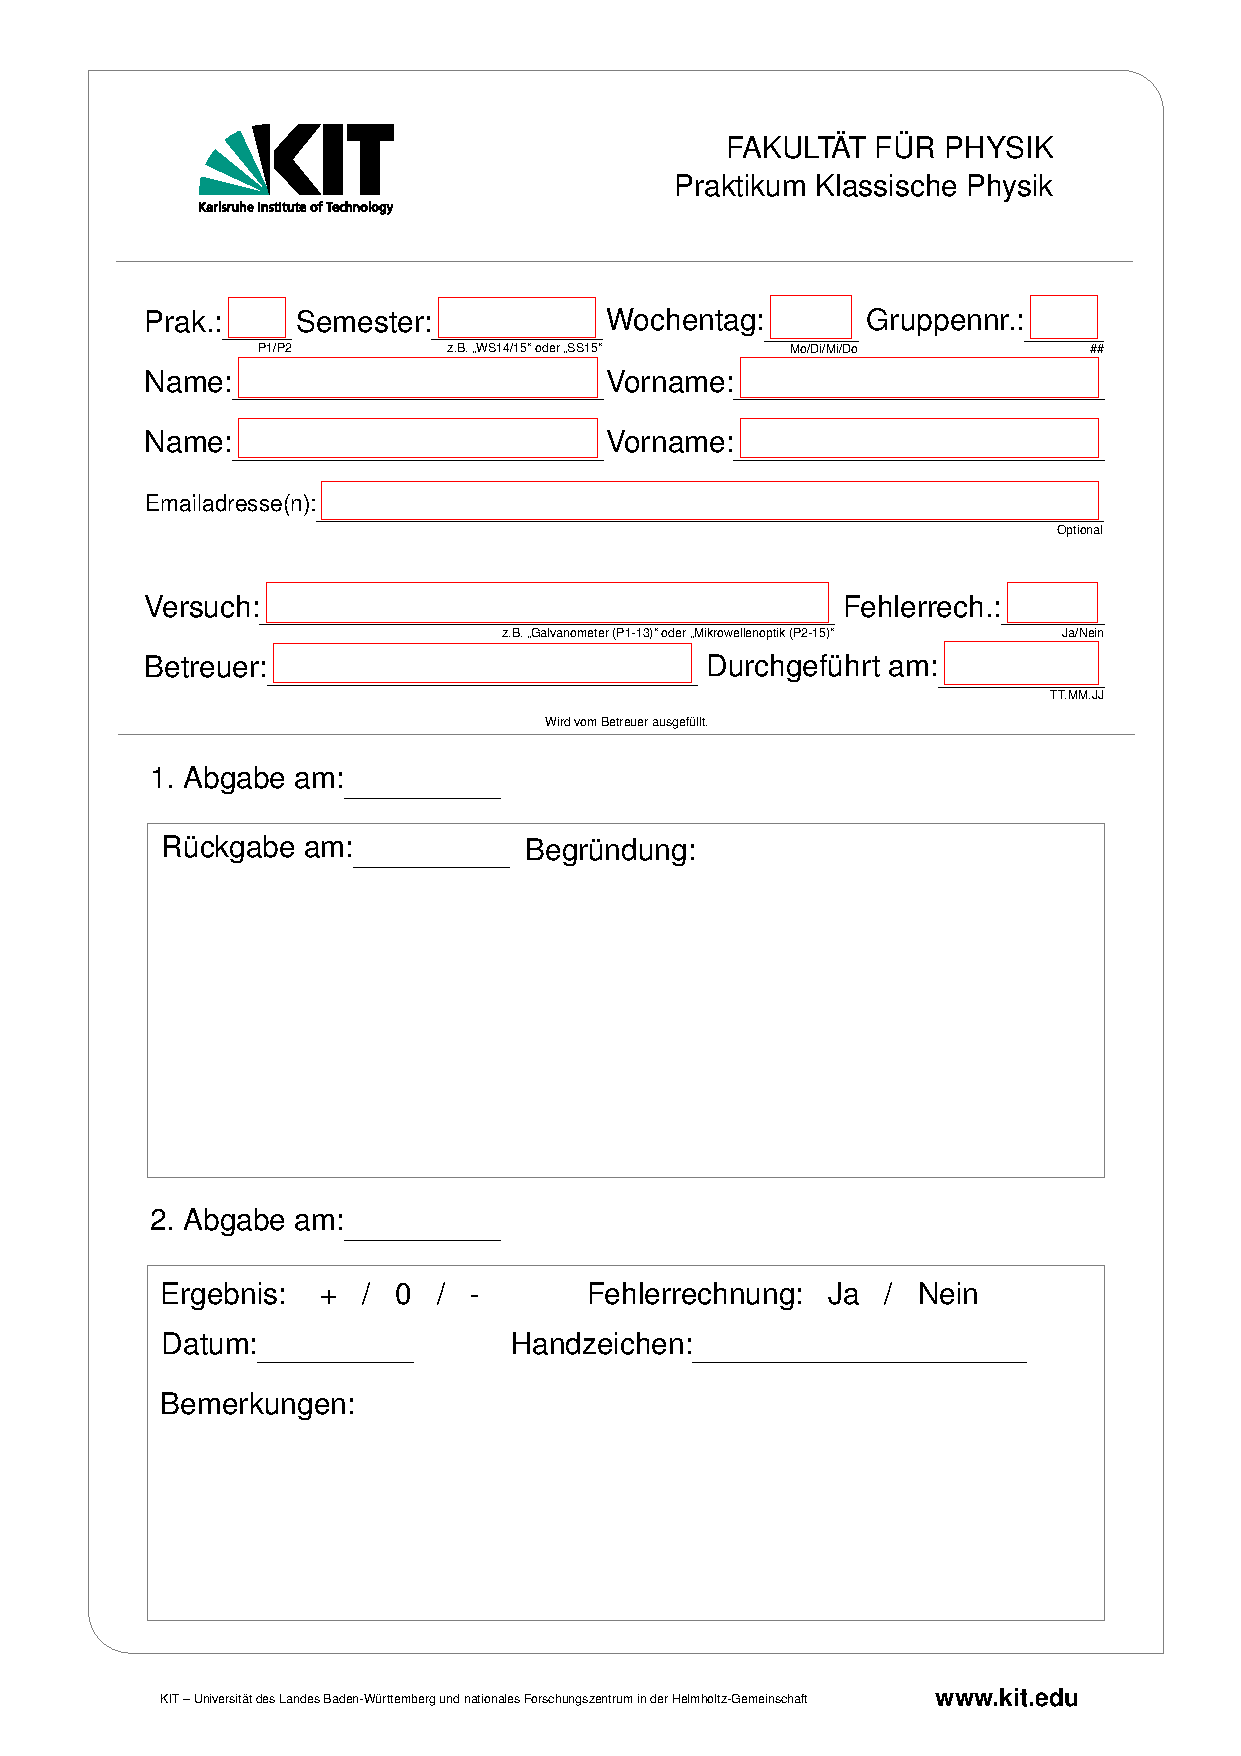
\includegraphics[page=1]{include/Deckblatt.pdf}};
    \begin{scope}[shift={(current page.south west)},every node/.style={anchor=base west}]
        % Grid to help find the positions (remove in final version)
        %\draw [help lines] (0,0) grid (current page.north east);
        %\draw [help lines,thick] (0,0) grid [step=5cm] (current page.north east);
        %
        \node at (3.95cm,24.15cm) {\Large{}}; % Praktikum:
        \node at (7.5cm,24.15cm) {\Large{}}; % Semester:
        \node at (13.2cm,24.15cm){\Large{}}; % Wochentag-Gruppe:
        \node at (17.6cm,24.15cm){\Large{}};% Gruppennummer:
        \node at (4cm,23.1cm){\Large{}}; % Nachname1:
        \node at (4cm,22.1cm){\Large{}}; % Nachname2:
        \node at (12.5cm,23.1cm){\Large{}}; % Vorname1:
        \node at (12.5cm,22.1cm){\Large{}}; % Vorname2:
        \node at (5.4cm,21.1cm){\Large{}}; % E-Mail Adressen:
        \node at (4.5cm,19.3cm){\Large{}}; %Versuch:
        \node at (17.1cm,19.3cm){\Large{}}; % Fehlerrechnung:
        \node at (4.55cm,18.3cm){\Large{}}; % Betreuer:in:
        \node at (16cm,18.3cm){\Large{}}; % Durchgeführt am:
        \node at (5.9cm,16.4cm){\Large{}}; % 1. Abgabe am:
        \node at (6cm,15.2cm){\Large{}}; %Rückgabe am:
        \node at (5.8cm,8.9cm){\Large{}}; % 2. Abgabe am:
    \end{scope}
\end{tikzpicture}